\subsubsection{Iteration 4: Evaluation on Path Following}

In this iteration, the drone was designed to follow a predefined path consisting of three sequential stages: take-off to a target altitude, navigation to a designated waypoint, and return to the home position, as described in the evaluation strategy in \cref{fig:path_design}. A cascading PID control structure was applied.

\paragraph{Design}

During the execution of the path-following task, the drone's position, rotation, and raw joystick inputs were recorded. The evaluation focuses on four visual analyses: (1) jerk magnitude over time, defined as the time derivative of acceleration and computed as $J = \sqrt{j_x^2 + j_y^2 + j_z^2}$, to assess motion smoothness; (2) throttle and pitch signals over time to examine forward flight behavior; (3) yaw and roll signals over time to evaluate turning behavior; and (4) a 3D trajectory plot to verify whether the intended path was successfully followed.

\paragraph{Enactment}

The results are shown in \cref{fig:path_result}. The left figure illustrates the full trajectory of the drone, including take-off, navigation to the waypoint, and return to the home position. From top to bottom, the subplots present: jerk magnitude over time; throttle (blue) and pitch (orange) joystick inputs over time; and yaw (blue) and roll (green) inputs over time.

\begin{figure}[H]
    \caption{Path Following Task Result.}\label{fig:path_result}
    \centering
    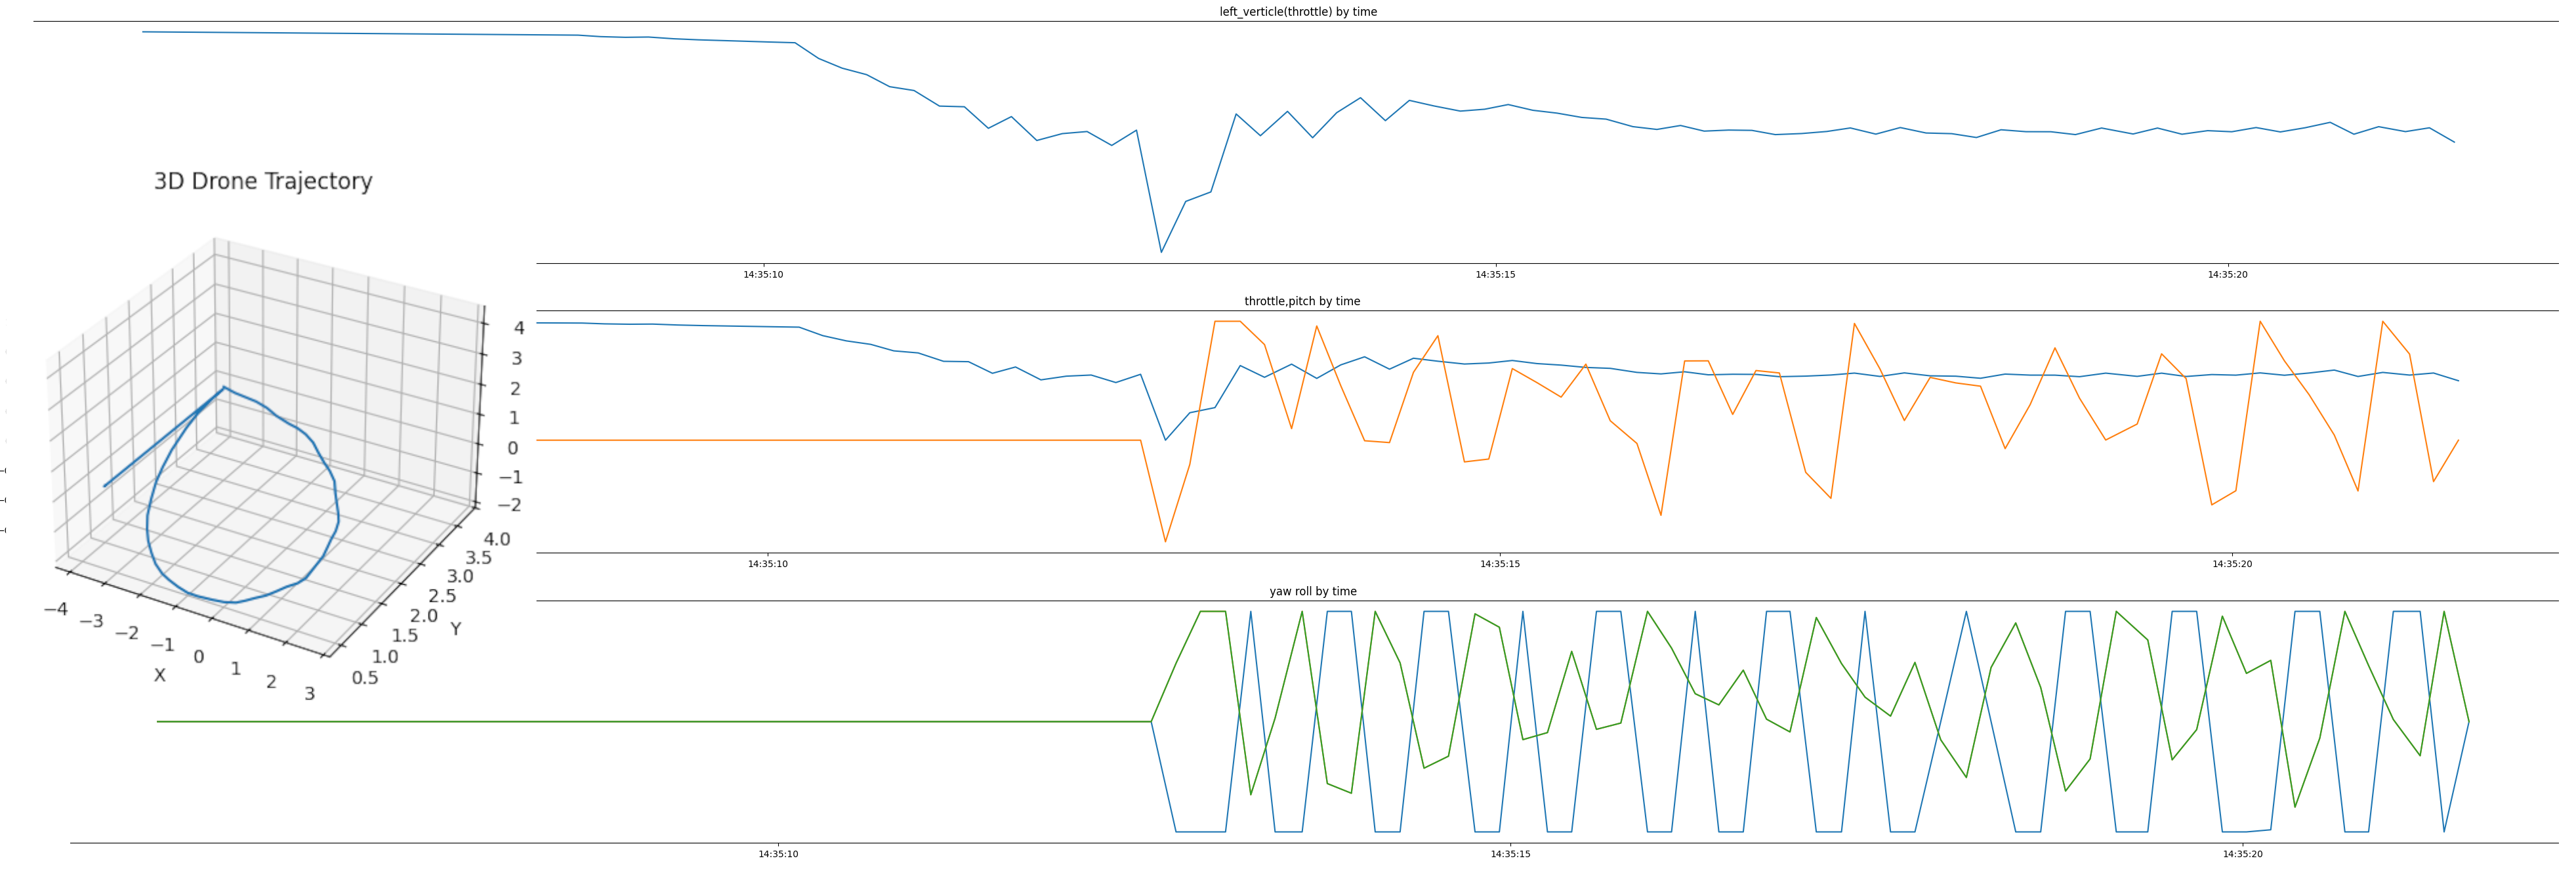
\includegraphics[width=1\linewidth]{img/path.png}
\end{figure}

\paragraph{Analysis}

As observed in the results in \cref{fig:path_result}, consistent with the previous iteration, the controller performs well during take-off and hovering phases. However, during forward flight, the pitch signal exhibits noticeable instability, occasionally taking negative values, indicating unintended backward motion. A similar issue can be seen during turning behavior, the bottom graph, where yaw and roll signals show inconsistent and negatively correlated patterns, whereas a positively correlated relationship would be expected under stable coordinated control.

Despite these instabilities, the system demonstrates sufficient functional performance for integration with the XR environment at its current stage of development.